\documentclass{article}

\usepackage[utf8]{inputenc}
\usepackage[spanish]{babel}
\usepackage{blindtext}
\usepackage{amsmath, amsthm, amsfonts}
\usepackage{latexsym, amssymb}
\usepackage{multicol}
% Set page size and margins
% Replace `letterpaper' with `a4paper' for UK/EU standard size
\usepackage[letterpaper,top=2cm,bottom=2cm,left=3cm,right=3cm,marginparwidth=1.75cm]{geometry}

\usepackage{natbib}
\usepackage[colorlinks=true, allcolors=blue]{hyperref}
\usepackage{url}

% Useful packages
\usepackage{amsmath}
\usepackage{graphicx}
\usepackage{pifont}
\usepackage[colorlinks=true, allcolors=blue]{hyperref}
\usepackage{icomma}
\usepackage{colortbl}
\usepackage{xcolor}
\usepackage[dvips]{graphicx, xcolor}

\definecolor{verde}{RGB}{133, 222, 148}
\definecolor{azul}{RGB}{195, 247, 203}


\renewcommand{\qedsymbol}{$\blacksquare$}
\theoremstyle{definition}
\newtheorem{prop}{Proposición}
\newtheorem{teor}{Teorema}
\newtheorem{defin}{Definición}
\newtheorem{obs}{Observación}
\newtheorem{ejem}{Ejemplo}
\newtheorem{nota}{Nota}

\title{Coeficientes binomiales descritos la perspectiva de la heurística matemática}
\author{Isaac Fabián Villa Miranda}
\date{27 de abril de 2024}

\begin{document}
\newcommand{\cbin}[2]{ \displaystyle \binom{#1}{#2} }

\maketitle

\section{Introducción} 
A partir de un conjunto con un cierto número de elementos, ¿cuántos subconjuntos de cardinalidad no mayor pueden formarse? ¿A qué patrón obedecen los coeficientes de la expansión de un binomio elevado a una potencia natural? ¿Existe siquiera tal patrón? ¿Por qué la suma de dichos coeficientes es siempre un cuadrado perfecto? Una característica que estos problemas tienen en común es que son resolubles sobre la base de un mismo ente matemático: los \textit{coeficientes binomiales}.
\section{Definición de \textit{coeficiente binomial}}
Un \textit{coeficiente binomial} es un número real (en particular, entero no negativo, de manera demostrable bajo ciertas restricciones) que, con base en distintas propiedades suyas, puede ser definido de dos maneras esencialmente idénticas. La definición presentada a continuación está a priori limitada a una propiedad algebraica característica, a partir de la cual puede ser derivada la otra definición, de índole combinatorio. Esta segunda definición, dada su importancia y su condición como resultado demostrable, será tratada como un teorema. 

La condición del coeficiente binomial como fruto de dos <<operandos>>, habitualmente llamados <<$n$>> y <<$k$>>, queda patente en sus distintas notaciones:

\begin{multicols}{7}
$ \binom{n}{k}$

$\displaystyle C(n,k)$

$\displaystyle _{n}C_{k}$

$\displaystyle ^{n}C_{k}$

$\displaystyle C^{k} _{n}$

$\displaystyle C^{n} _{k}$

$\displaystyle C_{n,k}$

\end{multicols}

\begin{defin}\label{def1}
Un coeficiente binomial $ \binom{n}{k}$ es igual a $\dfrac{n!}{k!(n-k)!}$ con $n \textnormal{, } k \in \mathbb{N}_{0}$ y $0 \leq k \leq n$. Si $k>n$ ó $k<0$, $ \binom{n}{k} := 0$.
\end{defin}

\begin{teor}
$\binom{n}{k}$ es el número de conjuntos de exactamente $k$ enteros elegidos cada uno entre 1, 2, 3, $\cdots$ , n.
\end{teor}
\begin{proof}[\textbf{{Demostración.}}]
Sean los conjuntos $A=\{1, 2, 3, \cdots , n\}$ y $B=\{a_{1}, a_{2}, a_{3}, \cdots , a_{k}\}$ tales que: $B\subseteq A$, $|A|=n$ y $|B|=k$.
Sin pérdida de generalidad: 
\begin{align*}
    a_{1}=1 \veebar a_{1}=2 \veebar a_{1}=3 \veebar \cdots \veebar a_{1}=n\\
      \Rightarrow  a_{2}=1 \veebar a_{2}=2 \veebar a_{2}=3 \veebar \cdots \veebar a_{2}=n,  &&a_{2}\neq a_{1}\\
       \Rightarrow     a_{3}=1 \veebar a_{3}=2 \veebar a_{3}=3 \veebar \cdots \veebar a_{3}=n,  &&a_{3}\neq a_{2}, && a_{3}\neq a_{1}\\
          \vdots\\
          \Rightarrow  a_{k}=1 \veebar a_{k}=2 \veebar a_{k}=3 \veebar \cdots \veebar a_{k}=n,  &&a_{k}\neq a_{j} \forall j \in [1,k-1] \cap \mathbb{N}.\\
\end{align*}
Así, si $\mathrm{Num}(x):=$ \textit{<<Cantidad de elementos de A que podrían ser iguales a $x \in B$>>}:
$$\mathrm{Num}(a_{1})=n\textnormal{, }  \mathrm{Num}(a_{2})=n-1\textnormal{, }  \mathrm{Num}(a_{3})=n-2\textnormal{,} \cdots \textnormal{, }  \mathrm{Num}(a_{k})=n-(k-1)=n-k+1. $$
De esta forma, el número de subconjuntos $B$ de $A$ que podrían formarse es:
$$\dfrac{\displaystyle \prod_{j=1}^{k} \mathrm{Num}(a_{j})}{k!}$$.

Simplificando la expresión:
$$\dfrac{\displaystyle \prod_{j=1}^{k} \mathrm{Num}(a_{j})}{k!}=\dfrac{\displaystyle \prod_{j=0}^{k-1}(n-j)}{k!}=\dfrac{n(n-1)(n-2)\cdots (n-k+1)}{k!}=\dfrac{\dfrac{n!}{(n-k)!}}{k!}=\dfrac{n!}{k!(n-k)!}= \displaystyle \binom{n}{k} \because \ref{def1}.$$
\end{proof}
Este resultado, adicionalmente, prueba que $\binom{n}{k}$ es un número natural cuando $n \textnormal{, } k \in \mathbb{N}_{0}$ y $0 \leq k \leq n$.
\section{Propiedades interesantes}
Una propiedad importante del coeficiente binomial es que puede ser expresado en términos de la suma de otros dos coeficientes binomiales con argumentos no mayores que los del coeficiente binomial inicial. En particular:
\begin{teor}
$\displaystyle\binom{n+1}{k}=\displaystyle\binom{n}{k-1}+\displaystyle\binom{n}{k}.$
\end{teor}
\begin{proof}[\textbf{{Demostración.}}]
\begin{align*}
    \cbin{n}{k-1}+\cbin{n}{k} &= \dfrac{n!}{(n-k+1)!(k-1)!}+\dfrac{n!}{(n-k)!k!}\\ &=\dfrac{n!k+n!(n-k+1)}{(n-k+1)!k!}\\ &=\dfrac{n!k+n!n-n!k+n!}{(n+1-k)!k!} \\ &= \dfrac{n!(n+1)}{(n+1-k)!k!} \\ &= \dfrac{(n+1)!}{(n+1-k)!k!}\\ &= \cbin{n+1}{k}.
\end{align*}
\end{proof}

Otra propiedad importante subyace a una sumatoria de coeficientes binomiales más que a un coeficiente binomial individual. El patrón sobre el que versa esta propiedad puede ser entrevisto en la siguiente tabla:

\begin{center}
\begin{tabular}
{|c|c|} \hline
\rowcolor{verde}
$\mathbf{n}$ & $\mathbf{\displaystyle \sum_{k=0}^{n} \cbin{n}{k}}$\\
\hline \hline
\rowcolor{azul} 0 & 1\\
\hline
\rowcolor{azul} 1 & 2\\
\hline
\rowcolor{azul} 2& 4\\
\hline
\rowcolor{azul} 3& 8\\
\hline
\rowcolor{azul} 4& 16\\
\hline
\rowcolor{azul} 5& 32\\
\hline
\rowcolor{azul} 6& 64\\
\hline
\rowcolor{azul} 7& 128\\
\hline
\rowcolor{azul} $\vdots$ & $\vdots$\\
\hline


   
\end{tabular}
\end{center}
La evidente conjetura que la tabla permite concebir puede ser demostrada por inducción y es, de hecho, cierta.
\begin{teor}
$\displaystyle \sum_{j=0}^{n} \cbin{n}{j}=2^n.$
\end{teor}\label{teo3}
\begin{proof}[\textbf{{Demostración.}}]
Primero, sea la proposición $P(x)$ definida como sigue: 
$$P(x):\displaystyle \sum_{j=0}^{x} \cbin{x}{j} = 2^{x}.$$
\begin{description}
\item[Caso base:] $P(0)$ es cierta porque:
\begin{align*}
\displaystyle \sum_{j=0}^{0} \cbin{0}{j} &= \cbin{0}{0} \\
&= \dfrac{0!}{0!(0-0)!}\\ &= 1 \because (0!=1)\\ &= 2^{0}.
\end{align*}
\item[Hipótesis de inducción:] $\exists n \in \mathbb{N}_{0} : P(n).$
\item[Demostración de $\mathbf{P(n+1)}$:] 
\begin{align*}
2^{n}  &= \displaystyle \sum_{j=0}^{n} \cbin{n}{j} \\
\Rightarrow 2^{n+1} &= 2\sum_{j=0}^{n} \cbin{n}{j} \\
&= \sum_{j=0}^{n} \cbin{n}{j} + \sum_{j=0}^{n} \cbin{n}{j}\\
&= \biggl[\sum_{j=0}^{n} \cbin{n}{j} + \cbin{n}{n+1}\biggr] + \biggl[\sum_{j=0}^{n} \cbin{n}{j} + \cbin{n}{-1}\biggr]  \because \biggl[\displaystyle\binom{m}{k}=0  \; \;  \forall \textnormal{ entero } k \notin [0,m].\biggr]\\
&= \sum_{j=0}^{n+1} \cbin{n}{j} + \sum_{j=-1}^{n} \cbin{n}{j} \\
&= \sum_{j=0}^{n+1} \cbin{n}{j} + \sum_{j=0}^{n+1} \cbin{n}{j-1}\\
&= \sum_{j=0}^{n+1} \cbin{n+1}{j} \because \biggl[\displaystyle\binom{m+1}{k}=\displaystyle\binom{m}{k-1}+\displaystyle\binom{m}{k}.\biggr] \\
&\therefore P(n+1).
\end{align*}

De la demostración exitosa de $P(n+1)$ a partir de la hipótesis $P(n)$ y el caso base $P(0)$, se desprende que la conjetura es cierta.
\end{description}
\end{proof}
\paragraph{}
\paragraph{}

\section{El teorema del binomio}
Hasta ahora no se había dado una explicación sobre la razón del nombre \textsl{coeficiente binomial}. El teorema presentado en esta sección puede implícitamente dilucidar el asunto. Para ello, merece la pena observar la siguiente tabla y los siguientes diagramas:
\begin{center}
\begin{tabular} 
{|c|c|c|c|} \hline
\rowcolor{verde}
$\mathbf{n}$ & $(a+b)^{n}$  & Expansión de $(a+b)^{n}$ & Coeficientes de la expansión, de izquierda a derecha\\
\hline \hline
\rowcolor{azul} 0 & $(a+b)^{0}$ & $1$ & $1$\\
\hline
\rowcolor{azul} 1 & $(a+b)^{1}$ & $a+b$ & $1 \textnormal{, }1$\\
\hline
\rowcolor{azul} 2 & $(a+b)^{2}$ & $a^2+2ab+b^2$ & $1 \textnormal{, }2 \textnormal{, 1}$\\
\hline
\rowcolor{azul} 3 & $(a+b)^{3}$ & $a^3+3a^{2}b+3ab^{2}+b^3$ & $1 \textnormal{, }3 \textnormal{, }3 \textnormal{, }1 $\\
\hline
\rowcolor{azul} 4 & $(a+b)^{4}$ & $a^4+4a^{3}b+6a^{2}b^{2}+4ab^3+b^{4}$ & $1 \textnormal{, }4 \textnormal{, }6 \textnormal{, }4 \textnormal{, }1 $\\
\hline
\rowcolor{azul} 5 & $(a+b)^{5}$ & $a^5+5a^{4}b+10a^{3}b^{2}+10a^{2}b^{3}+5ab^4+b^{5}$ & $1 \textnormal{, }5 \textnormal{, }10 \textnormal{, }10 \textnormal{, }5 \textnormal{, }1 $\\
\hline
\rowcolor{azul} $\vdots$ & $\vdots$ & $\vdots$ & $\vdots$\\
\hline
   
\end{tabular}
\end{center}

\begin{multicols}{2}


\begin{center}
\begin{tabular}
{c}
$\cbin{0}{0}$\\
\end{tabular}

\begin{tabular}
{c c}
$\cbin{1}{0}$ & $\cbin{1}{1}$\\
\end{tabular}

\begin{tabular}
{c c c}
$\cbin{2}{0}$ & $\cbin{2}{1}$ & $\cbin{2}{2}$\\
\end{tabular}

\begin{tabular}
{c c c c}
$\cbin{3}{0}$ & $\cbin{3}{1}$ & $\cbin{3}{2}$ & $\cbin{3}{3}$\\
\end{tabular}

\begin{tabular}
{c c c c c}
$\cbin{4}{0}$ & $\cbin{4}{1}$ & $\cbin{4}{2}$ & $\cbin{4}{3}$ & $\cbin{4}{4}$\\
\end{tabular}

\begin{tabular}
{c c c c c c}
$\cbin{5}{0}$ & $\cbin{5}{1}$ & $\cbin{5}{2}$ & $\cbin{5}{3}$ & $\cbin{5}{4}$ & $\cbin{5}{5}$\\ 
\reflectbox{$\ddots$} & \reflectbox{$\ddots$} &  &  & $\ddots$ & $\ddots$\\ 
\end{tabular} 


\paragraph{}
Coeficientes binomiales $\binom{n}{k}$ ordenados en filas según $n$ y en orden ascendente de izquierda a derecha según $0 \leq k \leq n$. Este diagrama es conocido como \textsl{triángulo de Pascal} o \textsl{triángulo de Tartaglia}.

\end{center}
 \vfill\null
\columnbreak

\begin{center}
\begin{tabular}
{c}
$1$\\
\end{tabular}

\begin{tabular}
{c c}
$1$ & $1$\\
\end{tabular}

\begin{tabular}
{ c c c}
$1$ & $2$ & $1$\\
\end{tabular}

\begin{tabular}
{c c c c}
$1$ & $3$ & $3$ & $1$\\
\end{tabular}

\begin{tabular}
{c c c c c}
$1$ & $4$ & $6$ & $4$ & $1$\\
\end{tabular}

\begin{tabular}
{c c c c c c}
$1$ & $5$ & $10$ & $10$ & $5$ & $1$\\
\reflectbox{$\ddots$} & \reflectbox{$\ddots$} &  &  & $\ddots$ & $\ddots$\\

\end{tabular}

\paragraph{}
Triángulo de Pascal simplificado.

\end{center}
\end{multicols}
Es llamativa la semejanza entre los coeficientes de la expansión binomial de $(a+b)^n$ y los números de la $n$-ésima fila del triángulo de Pascal. Esta es la motivación para la siguiente demostración por inducción.
\begin{teor}[\textbf{Teorema del binomio}] $$\forall a \textnormal{, } b \in \mathbb{R}\setminus \{0\} \; \; \forall n \in \mathbb{N}_0 : (a+b)^n= \displaystyle \sum_{k=0}^{n} \cbin{n}{k} a^{n-k}b^{k}.$$
\end{teor}
\begin{proof}[\textbf{Demostración}]
Primero, sea la proposición $P(x)$, evidentemente distinta de la existente en la demostración del teorema \ref{teo3}, definida como sigue:
$$P(x) \Leftrightarrow \forall a \textnormal{, } b \in \mathbb{R}\setminus \{0\} :(a+b)^x= \displaystyle \sum_{k=0}^{x} \cbin{x}{k} a^{x-k}b^{k}.$$
\begin{description}
\item[Caso base:] P(0) es cierta porque:
\begin{align*}
(a+b)^0 &= 1 \\
&= a^{0}b^{0} \\
&= a^{0-0}b^{0} \\
&= \displaystyle \sum_{k=0}^{0} \cbin{0}{k} a^{0-k}b^{k}.\\
\end{align*}
\item[Hipótesis de inducción:] $\exists n \in \mathbb{N}_0 : P(n).$
\item[Demostración de $\mathbf{P(n+1)}$:]

\begin{align*}
(a+b)^{n} &= \sum_{j=0}^{n} \cbin{n}{j} a^{n-j}b^{j} \\
\Rightarrow  (a+b)^{n+1} &= (a+b) \sum_{j=0}^{n} \cbin{n}{j} a^{n-j}b^{j} \\
&= \sum_{j=0}^{n} \cbin{n}{j} a^{n+1-j}b^{j} + \sum_{j=0}^{n} \cbin{n}{j} a^{n-j}b^{j+1} \\
&= \sum_{j=0}^{n} \cbin{n}{j} a^{n+1-j}b^{j} + \cbin{n}{n+1} a^{n+1-(n+1)}b^{n+1} + \sum_{j=1}^{n+1} \cbin{n}{j-1} a^{n-(j-1)}b^{(j-1)+1} \\
&= \sum_{j=0}^{n+1} \cbin{n}{j} a^{n+1-j}b^{j} + \sum_{j=1}^{n+1} \cbin{n}{j-1} a^{n+1-j}b^{j} + \cbin{n}{-1} a^{n+1-0}b^{0} \\
&= \sum_{j=0}^{n+1} \cbin{n}{j} a^{n+1-j}b^{j} + \sum_{j=0}^{n+1} \cbin{n}{j-1} a^{n+1-j}b^{j} \\
&= \sum_{j=0}^{n+1} \biggl[ \cbin{n}{j} a^{n+1-j}b^{j} + \cbin{n}{j-1} a^{n+1-j}b^{j} \biggr] \\
&= \sum_{j=0}^{n+1} \biggl\{ \biggl[ \cbin{n}{j} + \cbin{n}{j-1} \biggr] a^{n+1-j}b^{j} \biggr\} \\
&= \sum_{j=0}^{n+1}  \cbin{n+1}{j}  a^{n+1-j}b^{j}.\\
&\therefore P(n+1).
\end{align*}
\end{description}
La demostración de $P(n+1)$ concluye la demostración del teorema.
\end{proof}

\clearpage
\section{Propiedades geométricas asociadas}
El teorema del binomio tiene la siguiente representación geométrica para valores pequeños de $n$:
\begin{figure}[!htbp]
\begin{center}
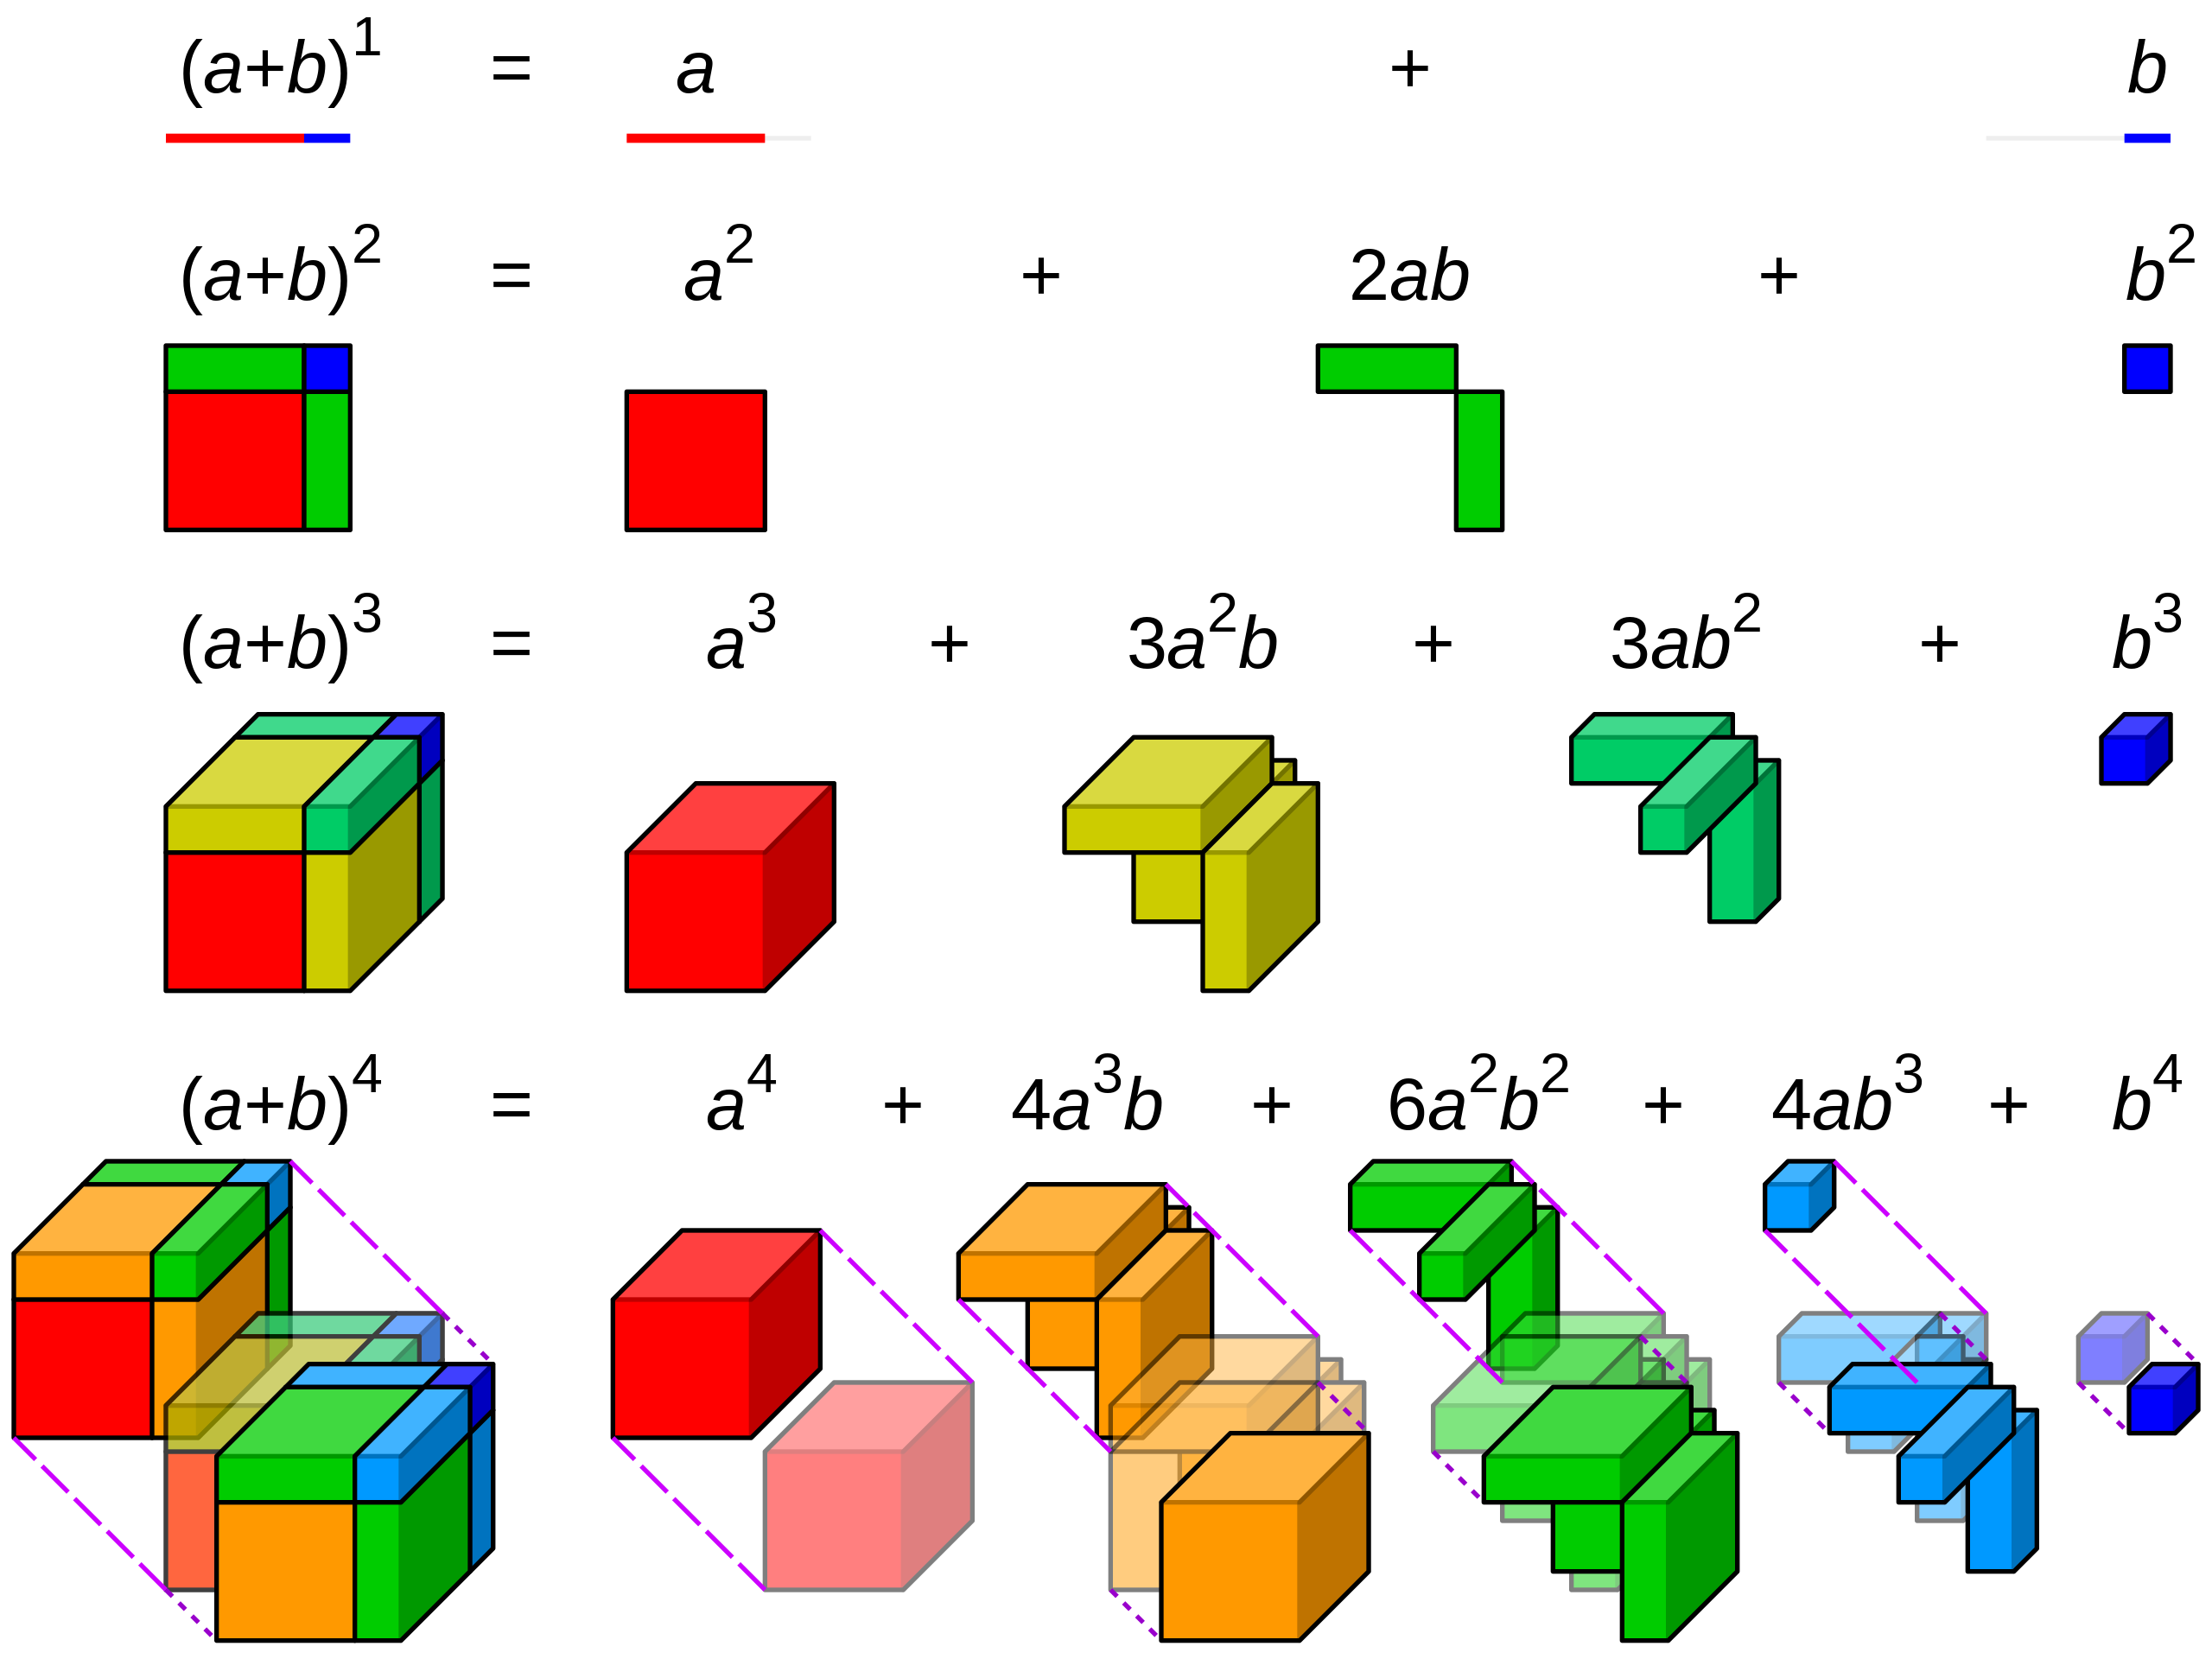
\includegraphics[scale=0.06]{binomial1.png}
\caption{\citep{misc1}}
\end{center}
\end{figure}



Por otra parte, dada una distinción visual entre números según su paridad, un triángulo de Pascal puede acabar asemejándose a un triángulo de Sierpinski: un fractal constituido por infinitos triángulos equiláteros. En genéral, la distinción visual de los números del triángulo de Pascal según su congruencia módulo $p$, con $p$ primo, siempre acaba generando un fractal. 
\citep{1708.07429}

\begin{figure}[!htbp]
\begin{center}
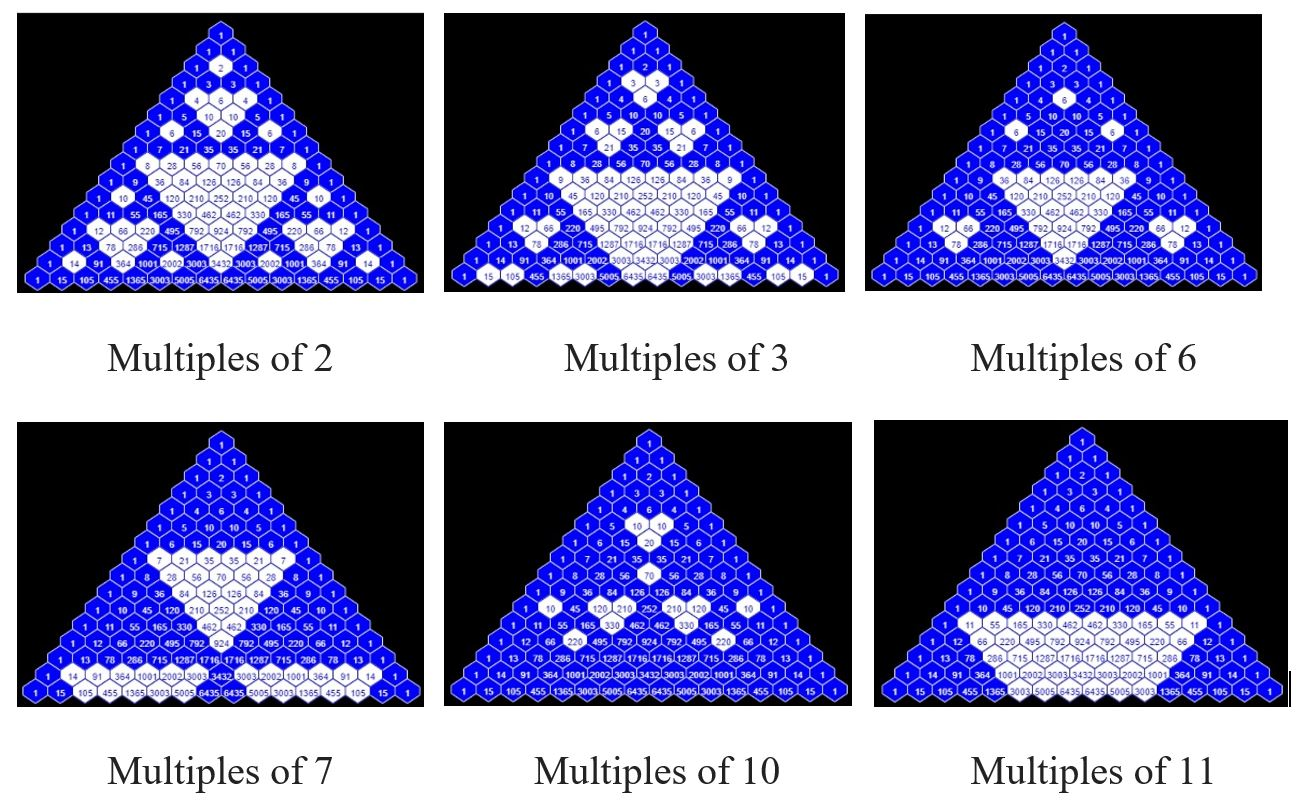
\includegraphics[scale=0.51]{pascal1.jpg}
\caption{Múltiplos de $p \leq 11$ resaltados en el triángulo de Pascal. Todos los triángulos tienen quince filas. \citep{Pascal}}
\end{center}
\end{figure}



\begin{figure}[!htbp]
\begin{center}
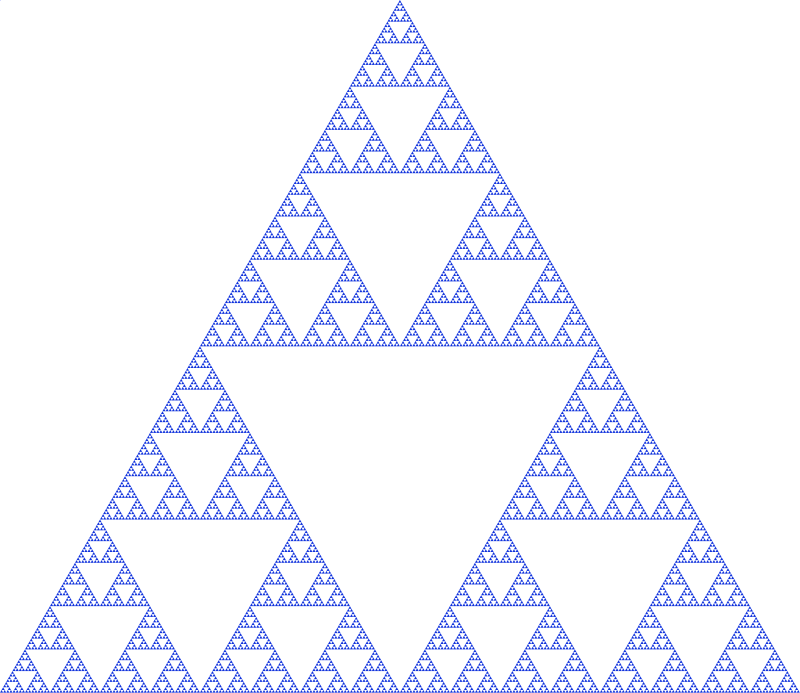
\includegraphics[scale=0.2]{spin2.png}
\caption{Un triángulo de Sierpinski. \citep{wiki:xxx}}
\end{center}
\end{figure}


\clearpage\bibliographystyle{plain}
\bibliography{sample}

\end{document}
